\documentclass[journal]{IEEEtran}
\usepackage[T1]{fontenc}
\usepackage{mathptmx}
\usepackage{amsmath,amssymb,graphicx,booktabs,cite,float,url}
\setlength{\textfloatsep}{10pt plus 2pt minus 2pt}
\setlength{\dbltextfloatsep}{10pt plus 2pt minus 2pt}
\setlength{\dblfloatsep}{8pt plus 2pt minus 2pt}
\setlength{\intextsep}{8pt plus 2pt minus 2pt}
\raggedbottom
\hyphenation{multi-modal land-slide back-scatter}
\makeatletter\newcommand{\rows}[1]{\@@input #1 }\makeatother  % expandable input for table rows
\newcommand{\oursAP}{77.59}
\newcommand{\oursIoU}{56.45}
\newcommand{\oursFone}{72.17}
\newcommand{\oursInd}{69.46}
\newcommand{\oursSpt}{49.88}
\newcommand{\oursP}{74.2}
\newcommand{\oursR}{70.3}

\begin{document}
\title{Cross-Event Optical Relation Distillation for SAR Landslide Mapping}
\author{Jiuqi~Zhang, Jili~Wang, Heng~Zhang, and Yi~Zhang%
\thanks{Jiuqi Zhang, Jili Wang, and Heng Zhang are with the Department of Space Microwave Remote Sensing System, Aerospace Information Research Institute, Chinese Academy of Sciences, Beijing 100190, China, and also with the School of Electronic, Electrical and Communication Engineering, University of Chinese Academy of Sciences, Beijing 100039, China (e-mail: zhangjiuqi23@mails.ucas.ac.cn; wangjl01@aircas.ac.cn; zhangheng@aircas.ac.cn).}
\thanks{Yi Zhang is with the School of Electronic, Electrical and Communication Engineering, University of Chinese Academy of Sciences, Beijing 100039, China (e-mail: zhangyi@aircas.ac.cn).}
\thanks{Corresponding author: Jili Wang (e-mail: wangjl01@aircas.ac.cn).}
}
\IEEEaftertitletext{\vspace{-3pt}}

\maketitle

\begin{abstract}
Rapid post-disaster landslide mapping supports damage assessment and emergency response. Optical imagery provides useful surface-change information, but cloud cover can limit its availability when a map is needed. We use optical observations during training to improve mapping from synthetic aperture radar (SAR) and terrain data at deployment. We propose cross-event optical relation distillation, which transfers the distribution of regional similarities from a frozen optical--SAR teacher to a SAR student. For each region, teacher and student similarities to regions of other disaster events are sorted independently and matched using a one-dimensional Wasserstein loss. This preserves distributional guidance without requiring the same region pairs to have the same similarity. A bank of learnable prototypes shared across three decoder scales refines the student features and remains available at inference. On the official DLR Sentinel-1/2 split, the method achieves 56.45\% pixel-pooled intersection over union (IoU) and 77.59\% average precision, compared with 52.20\% and 72.91\% for the U-Net baseline. Deployment requires pre- and post-event SAR, elevation, and slope, with no optical input.
\end{abstract}

\begin{IEEEkeywords}
Knowledge distillation, landslide mapping, privileged information, synthetic aperture radar (SAR), Sentinel-2.
\end{IEEEkeywords}

\section{Introduction}
Early maps of disaster-triggered landslides help identify affected slopes and support damage assessment and emergency response~\cite{Mondini2021,Handwerger2022,Amatya2023}. Optical observations reveal surface changes associated with slope failure, but clouds and illumination conditions can restrict timely coverage. Synthetic aperture radar (SAR) supplies an alternative under these conditions, and neural networks have demonstrated its potential for landslide mapping~\cite{Nava2022DL,Nava2022Attention,Boehm2022}. The DLR multi-sensor benchmark nevertheless reports a substantial difference between optical and SAR performance~\cite{Orynbaikyzy2025}. We therefore ask whether optical observations available in training archives can improve a mapper that uses pre- and post-event SAR and terrain data when optical observations are unavailable.

Learning with privileged information and knowledge distillation provide a framework for this asymmetric availability~\cite{LopezPaz2016,Hinton2015}. A teacher with richer inputs supervises a student whose deployment inputs are restricted. Existing approaches transfer predictions, attention, or intermediate features~\cite{Zagoruyko2017,Lan2025ACAM,Kieu2026DIS2,Sun2027}. Relational approaches instead transfer similarities between examples or representations~\cite{Park2019RKD,Tung2019SP}; PKDOT uses optimal transport to transfer privileged multimodal relational information~\cite{Aslam2024PKDOT}. These alternatives motivate examining which aspect of an optical teacher's representation is useful to a SAR student.

Landslide inventories group observations by disaster event, with variation in terrain, vegetation, and acquisition conditions. Performance on validation patches from training events can therefore differ from performance on other events. Moreover, matching optical features directly may constrain a student to reproduce modality-specific responses. In our experiments, closer agreement with selected teacher region pairs does not consistently accompany higher test accuracy. This observation motivates a less restrictive target: the distribution of similarities to regions from other events, while allowing teacher and student to assign those similarities to different partners. It does not assume that all optical information is recoverable from SAR.

We propose cross-event optical relation distillation with a prototype-enhanced U-Net student. The teacher uses optical, SAR, and terrain inputs during training; the deployed student uses SAR and terrain alone. A Wasserstein loss matches independently sorted cross-event similarity distributions at one decoder stage. A shared prototype bank refines three decoder scales, coupling the representation trained by this loss to finer-resolution features. Segmentation comparisons, component and stage ablations, and per-event analysis assess the resulting accuracy, the contribution of each design, and the variation across landslide events.

\section{Method}
\subsection{Problem Formulation}
Let $X_s$ denote the student input: pre- and post-event Sentinel-1 $\gamma^0$ VV/VH backscatter, elevation, and slope (six channels). The teacher additionally receives pre- and post-event Sentinel-2 bands $X_o$ (twelve channels). Both networks follow the U-Net of~\cite{Orynbaikyzy2025,Ronneberger2015}, with four decoder stages whose feature maps measure $16\times16$, $32\times32$, $64\times64$, and $128\times128$ for a $128\times128$ input, so that one feature cell spans 80, 40, 20, and 10~m. The teacher is trained with the segmentation loss and then frozen; the student is trained with the teacher and deployed on $X_s$ only. Fig.~\ref{fig:method} summarizes the method.

\begin{figure*}[!t]
\centering
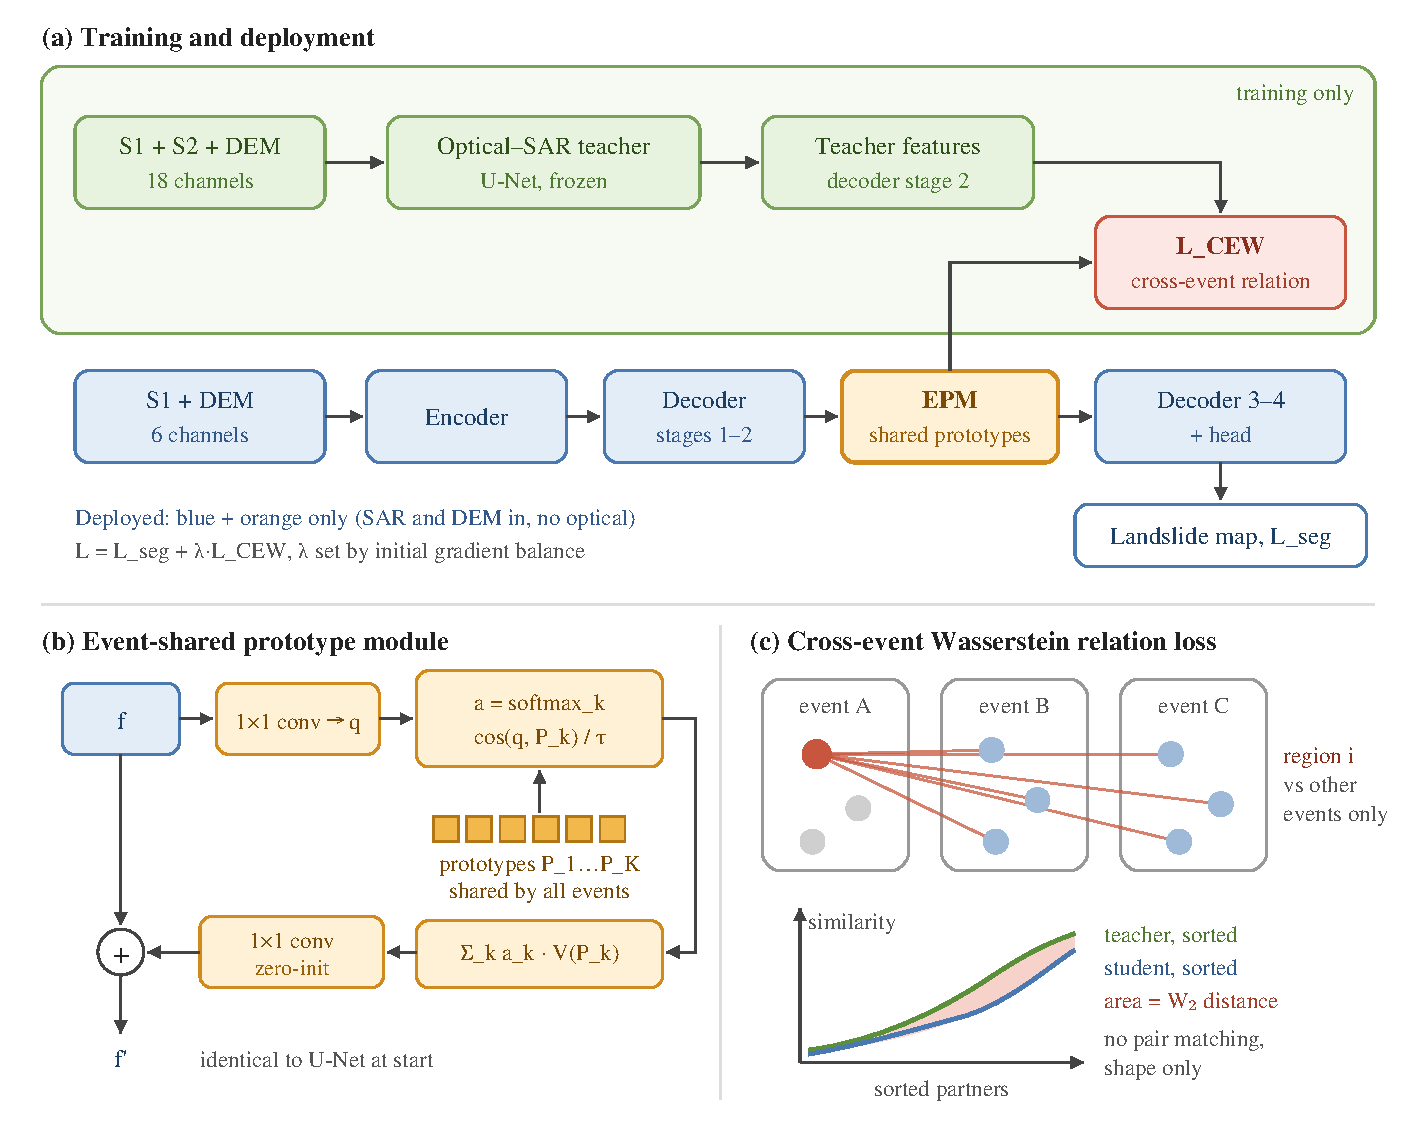
\includegraphics[width=0.98\textwidth]{figures_dlr/method.pdf}
\caption{(a) Frozen optical--SAR teacher and SAR--terrain student with U-Net skip connections. EPMs refine three decoder scales; relation supervision uses only the 32-pixel stage. (b) Shared-prototype refinement with stage-specific projections and residual addition. (c) Per-anchor matching of independently sorted cross-event similarities. Gray blocks exclude same-event pairs; matrix entries and bars are schematic.}
\label{fig:method}
\end{figure*}

\subsection{Scale- and Event-Shared Prototypes}
After decoder stage $l\in\{2,3,4\}$ (feature maps of $32$, $64$, and $128$ pixels per side), the student feature $f_l\in\mathbb{R}^{C_l\times H_l\times W_l}$ is compared with one bank of $K$ learnable prototypes $\{P_k\}$ shared by all events and stages:
\begin{equation}
a_{lk}(p)=\mathrm{softmax}_k\!\left(\cos\bigl(W_q^l f_l(p),P_k\bigr)/\tau\right),
\label{eq:assign}
\end{equation}
\begin{equation}
f_l'(p)=f_l(p)+W_o^l\sum_k a_{lk}(p)\,W_v^l\hat P_k ,
\label{eq:refine}
\end{equation}
where $\hat P_k=P_k/\|P_k\|_2$, $p$ indexes a feature location, $W_q^l$, $W_v^l$, and $W_o^l$ are stage-specific $1\times1$ projections, $\tau=0.1$, and $K=16$. $W_o^l$ is zero-initialized, so training starts from the plain U-Net. Sharing the bank couples the three stages without requiring identical stage-specific projections. The relation loss can update this common bank through stage 2, while segmentation supervision trains all stages; sharing alone does not guarantee event-invariant features. The prototypes remain in the deployed network.

\subsection{Cross-Event Wasserstein Relation Distillation}
The relation loss acts at stage 2 ($32\times32$ feature map). Teacher and refined student features there are average-pooled over valid pixels into $4\times4$ regions per patch, each covering $320\times320$~m, with at least 75\% valid coverage and normalized to unit length, giving $t_i$ (teacher) and $s_i$ (student, from $f_2'$). For region $i$ from event $e_i$, let $\mathcal{N}_i=\{j: e_j\neq e_i\}$ be the regions of other events in the mini-batch. The teacher and student similarity sets are
\begin{equation}
\mathcal{T}_i=\{t_i^\top t_j\}_{j\in\mathcal{N}_i},\qquad \mathcal{S}_i=\{s_i^\top s_j\}_{j\in\mathcal{N}_i},
\end{equation}
each shifted by its minimum over all cross-event pairs in the batch. Sorting each set separately gives $\tilde{\mathcal{T}}_i$ and $\tilde{\mathcal{S}}_i$, and the squared one-dimensional Wasserstein distance between the two empirical distributions is
\begin{equation}
L_{\mathrm{CEW}}=\frac{1}{N}\sum_{i=1}^{N}\frac{1}{|\mathcal{N}_i|}\sum_{r=1}^{|\mathcal{N}_i|}\bigl(\tilde{\mathcal{T}}_i[r]-\tilde{\mathcal{S}}_i[r]\bigr)^2 .
\label{eq:cew}
\end{equation}
Regions with fewer than two cross-event partners are excluded, and $N$ counts retained anchor regions. Sorting removes partner correspondence: the student decides which regions of other events are close or distant, while the teacher prescribes how the cross-event similarities are distributed. Same-event pairs are excluded to reduce direct matching of within-event structure. The loss does not explicitly remove event information, and retains the geographic correspondence of the anchor region. No top-$k$ partner count or quantile count is required.

Stage 2 summarizes each region from $8\times8$ feature cells. Applying the relation loss here leaves finer stages supervised by segmentation while they share the prototype bank. Gradients from $L_{\mathrm{CEW}}$ update the student features, projections, and shared prototypes; teacher features are detached. Section~III-E evaluates the choice of stage.

\subsection{Learning Objective}
The student minimizes
\begin{equation}
L=L_{\mathrm{BCE}}+L_{\mathrm{Dice}}+\lambda L_{\mathrm{CEW}},
\label{eq:loss}
\end{equation}
with binary cross-entropy and foreground soft Dice on valid pixels. The reported configuration uses $\lambda=30$, $K=16$, and $\tau=0.1$. The teacher and $L_{\mathrm{CEW}}$ are removed after training.

\section{Experiments}
\subsection{Dataset and Settings}
We use the Sentinel-1/2 landslide reference data of~\cite{Orynbaikyzy2025} with its official split: 355 training and 88 validation patches from 23 events, and 120 test patches of $128\times128$ pixels at 10~m. The test set contains 44 patches from four independent events (Ind.) and 76 patches from four dependent events whose training patches are separated by a spatial block split (Dep.). Inputs follow the one-pre/one-post setting of~\cite{Orynbaikyzy2025}: $\gamma^0$ VV/VH in decibels, Copernicus DEM elevation, and slope; the teacher adds Sentinel-2 B2, B3, B4, B8, B11, and B12 from the pre- and post-event scenes.

All U-Nets, including the teacher and every student, use AdamW with a learning rate of $10^{-4}$, weight decay of 0.01, gradient clipping at 1, batches of 16, random flips and $90^\circ$ rotations, and 200 epochs (constant rate for 100 epochs, then cosine decay to 1\%). Validation IoU, computed every 20 epochs, selects the checkpoint; each model is tested once after selection, at threshold 0.5. All students share one initialization, one data order, and the same frozen teacher. We report AP and pixel-pooled IoU and F1 over the 120 test patches, IoU on Ind. and Dep., and per-event F1 as in~\cite{Orynbaikyzy2025}. Each configuration is one training run with seed 42.

\begin{figure*}[!t]
\centering
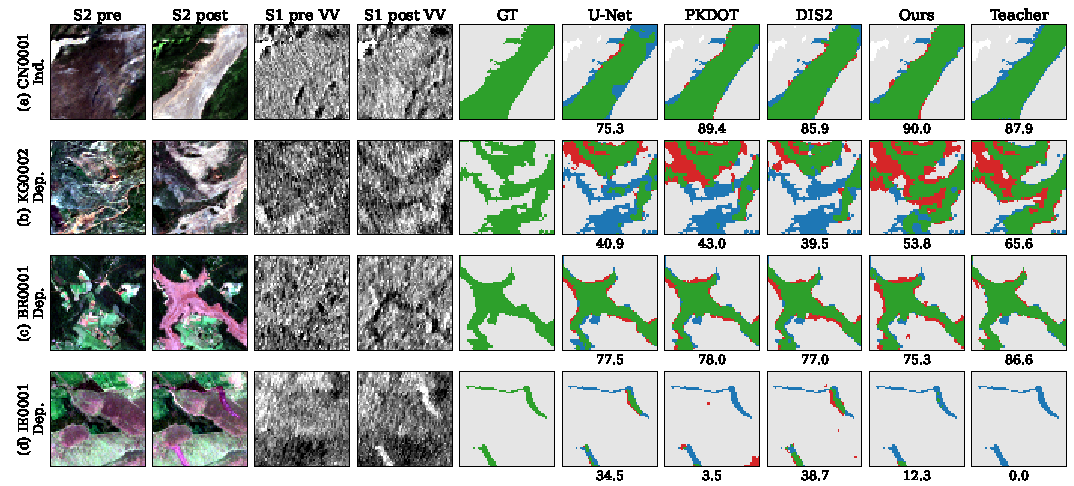
\includegraphics[width=\textwidth]{figures_dlr/qualitative.pdf}
\caption{Selected test patches with pre- and post-event Sentinel-2 reference images. Optical (true-color) and SAR panels show inputs; only the teacher receives the optical scenes. GT: reference (green). Predictions at threshold 0.5: true positives green, false positives red, false negatives blue; white marks invalid SAR pixels. Numbers give patch IoU (\%). (a), (b) cases where Ours changes the map; (c) all students are similar; (d) small peat slides that the teacher also misses.}
\label{fig:qualitative}
\end{figure*}

\subsection{Main Comparison}
\begin{table}[!t]
\caption{Test results (\%). Rows above the reference block receive SAR and terrain at inference. Distillation methods share the U-Net student, initialization, and frozen optical--SAR teacher. Bold: best SAR-input value.}
\label{tab:main}
\centering\footnotesize
\setlength{\tabcolsep}{3.5pt}
\begin{tabular}{@{}lrrrrr@{}}
\toprule
Method & AP & IoU & F1 & IoU Ind. & IoU Dep. \\
\midrule
\rows{tables_dlr/main_rows.tex}
\bottomrule
\end{tabular}
\end{table}

Table~\ref{tab:main} compares direct segmentation networks trained on the same input and recipe---the U-Net of~\cite{Orynbaikyzy2025} and UNet++ and DeepLabv3 with ImageNet ResNet-34 encoders~\cite{He2016ResNet}---with distillation methods that transfer outputs (Vanilla KD), attention or features (AT, Multi-to-Uni, ACAM-KD, DIS2), and pairwise relations (PKDOT). The compared distillation losses are adapted to the common U-Net student and frozen teacher; these are task adaptations rather than original-task benchmark results. Ours additionally includes the prototype modules. The ImageNet-initialized UNet++ and DeepLabv3 reach only 38.69\% and 44.20\% IoU despite 89.7\% and 84.5\% validation IoU, illustrating a substantial validation--test gap under this protocol. Ours improves IoU by 4.25 points and AP by 4.68 points over the U-Net, and gives the highest pooled AP, IoU, and F1 in the main comparison, 0.48 IoU points above DIS2 and 0.96 AP points above the best competing AP. The gain comes mainly from recall (\oursR\% versus 58.4\%), at lower precision (\oursP\% versus 83.1\%). On the independent events, PKDOT and DIS2 remain 1.06 and 0.25 points higher; Ours is highest on the dependent events. Vanilla KD raises IoU but reduces AP relative to the baseline. The optical-input references remain more accurate, showing a gap between access to optical observations at inference and training-only guidance.

Fig.~\ref{fig:qualitative} shows four selected test patches with optical reference images. On the rockslide in (a), Ours and PKDOT recover the margins that the U-Net misses. On the loess slides in (b), Ours recovers slopes that all other students miss, at the cost of additional false positives, similar to the teacher. In (c) all students produce similar maps. In (d), small peat slides are largely missed by all models, including the teacher.

\subsection{Per-Event Results}
\begin{table}[!t]
\caption{Test F1 (\%) per event and mean over the four independent (Ind.) and four dependent (Dep.) events.}
\label{tab:events}
\centering\footnotesize
\setlength{\tabcolsep}{2.2pt}
\begin{tabular}{@{}lrrrrrrrrrr@{}}
\toprule
& CN & CO & IN & PH & Ind. & BR & CA & IE & KG & Dep. \\
\midrule
\rows{tables_dlr/event_rows.tex}
\bottomrule
\end{tabular}
\end{table}

The dataset paper reports per-event F1 averaged over events rather than pooled scores; for $\gamma^0$ VV/VH with terrain it gives a mean F1 of 0.68 over the dependent events with its own training~\cite{Orynbaikyzy2025}. Under our recipe the U-Net reaches 62.3\% (Table~\ref{tab:events}). Ours raises F1 on the large Chinese rockslide (CN), the Philippine slides (PH), and the Kyrgyz loess slides (KG), but falls on the small Irish peat slides (IE), which the teacher misses entirely. This shared failure identifies a case in which the teacher supplies limited useful guidance; the comparison alone does not establish its cause. Averaged over events, Ours (59.1\%) is close to the U-Net (58.8\%) and below DIS2 (62.8\%); its advantage lies in pixel-pooled scores, which are dominated by the larger landslides.

\subsection{Analysis of Relational Transfer}
For every training and validation region we take the 30 regions of other events that the teacher finds least similar and measure the share that a frozen student also ranks among its own 30 least similar. Across 13 students trained with the same recipe, this agreement correlates negatively with test IoU ($r=-0.70$; Fig.~\ref{fig:overlap}). The best students agree with the teacher less than the U-Net does, whereas losses that enforce pair correspondence raise the agreement to 0.68--0.82 while test IoU falls to 52--53\%. This association motivates relaxing partner correspondence, but does not establish that pairwise transfer is generally ineffective or identify event memorization as its cause.

\begin{figure}[!t]
\centering
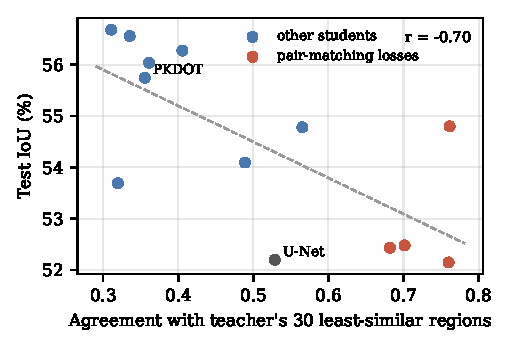
\includegraphics[width=\columnwidth]{figures_dlr/overlap.pdf}
\caption{Teacher--student agreement on the teacher's 30 least similar cross-event regions (validation patches) versus test IoU for students trained with the same recipe.}
\label{fig:overlap}
\end{figure}

\subsection{Ablation Study}
\begin{table}[!t]
\caption{Ablation (\%). All rows use the same U-Net, initialization, teacher, and recipe. Stages are named by feature-map size. $^\dagger$Repeating this run with identical settings gave 56.03\% IoU.}
\label{tab:ablation}
\centering\footnotesize
\setlength{\tabcolsep}{4pt}
\begin{tabular}{@{}lrrr@{}}
\toprule
Configuration & AP & IoU & IoU Ind. \\
\midrule
\rows{tables_dlr/ablation_rows.tex}
\bottomrule
\end{tabular}
\end{table}

Table~\ref{tab:ablation} isolates each component. $L_{\mathrm{CEW}}$ alone raises IoU from 52.20\% to 55.57\%. The shared prototypes alone have little effect on IoU (52.07\%) but raise AP to 77.99\%: they improve AP without improving pooled IoU at threshold 0.5. The combined model improves IoU by 0.88 points over the loss-only variant and achieves higher recall than the baseline. Separate prototypes at 32 and 64 pixels with the loss at both stages lower IoU to 55.22\% and independent-event IoU to 64.85\%, whereas one bank shared by three stages and constrained only at 32 pixels gives 56.45\% IoU. With the shared prototypes and the same $320$-m regions, moving $L_{\mathrm{CEW}}$ from the 32-pixel stage to the 16-, 64-, or 128-pixel stage lowers IoU to 55.57\%, 55.18\%, and 52.44\%, and applying it at all three prototype stages gives 54.31\%. Independent-event IoU falls from \oursInd\% at 32 pixels to 58.32\% at 128 pixels. These results favor the 32-pixel stage in this experiment; modality-specific fine-scale texture is a possible explanation, rather than a measured cause.

Losses that impose pair correspondence fall to 52.4--52.5\% IoU. Pairing each region with the teacher's 30 least similar partners and matching them by optimal transport (OT), as in PKDOT, and summarizing the distribution by 32 quantiles matched by OT reach scores similar to the Wasserstein distance (56.68\% and 56.55\%); the former repeated at 56.03\%. The Wasserstein form needs no partner count, quantile number, or iterative solver. The tested label-defined relation target trails the optical-teacher target by 1.65 points, supporting the latter under this comparison.

\begin{figure}[!t]
\centering
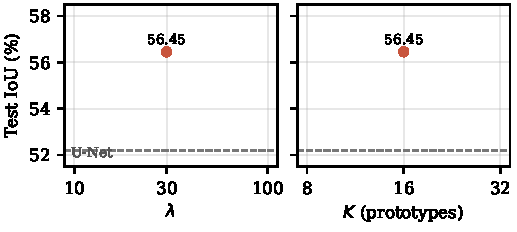
\includegraphics[width=\columnwidth]{figures_dlr/sensitivity.pdf}
\caption{Test IoU of Ours for the relation-loss weight $\lambda$ (left, $K=16$) and the number of prototypes $K$ (right, $\lambda=30$). Dashed line: U-Net. Reference configuration: $\lambda=30$, $K=16$.}
\label{fig:sensitivity}
\end{figure}

Fig.~\ref{fig:sensitivity} varies one setting at a time. With $\lambda=10$, AP remains high (78.52\%) but IoU drops to 54.06\%; with $\lambda=100$, validation IoU falls to 63.1\%, and test IoU (52.18\%) returns to the U-Net level. Eight and 32 prototypes give 54.91\% and 54.99\%. Except for $\lambda=100$, every tested setting stays at least 1.8 points above the U-Net.

\subsection{Deployment Cost}
\begin{table}[!t]
\caption{Deployed parameters and multiply--accumulate operations (MACs) for one $128\times128$ patch.}
\label{tab:cost}
\centering\footnotesize
\begin{tabular}{@{}lrr@{}}
\toprule
Network & Params (M) & MACs (G) \\
\midrule
\rows{tables_dlr/cost_rows.tex}
\bottomrule
\end{tabular}
\end{table}

All configurations are single runs; a repeated relational variant differed by 0.65 IoU points. Small differences between methods therefore require cautious interpretation. The official validation set shares events and overlapping spatial coverage with training; Ind. is event-disjoint, whereas the pooled test combines Ind. and Dep. The benchmark has also been used during earlier development, so the results are not a new blind evaluation.

The three prototype modules add 0.14\,M parameters and 0.36\,G MACs to the U-Net (about 3\% more MACs, Table~\ref{tab:cost}). The other distillation students deploy the unchanged U-Net. The teacher and $L_{\mathrm{CEW}}$ are used only in training, so inference uses SAR and terrain alone.

\section{Conclusion}
We presented cross-event optical relation distillation for landslide mapping from SAR and terrain inputs. A frozen optical--SAR teacher supervises distributions of cross-event regional similarities, and a shared prototype bank refines three student decoder scales. On the DLR benchmark, the method improves pixel-pooled IoU from 52.20\% to 56.45\% and AP from 72.91\% to 77.59\%. The improvement is strongest in pooled scores and recall; it does not extend to the best event-averaged performance. The deployed model uses no optical observations and adds 0.14 M parameters and 0.36 G MACs to the U-Net.

\bibliographystyle{template/IEEEtran}
\bibliography{references_dlr}
\end{document}
